%=====================================================================
\section{Which assumption matters most}
\label{sec:ranking}

Putting all seven experiments on one scale answers the operator's real question: where is it worth spending effort
to measure a number well, or money to change it?

\textbf{Effect on the total cost $Z$} (a $\pm25$\,\% or comparable change), largest first:
\begin{enumerate}[itemsep=1pt]
  \item \textbf{Charging demand} (E10): about $\pm22$\,\% --- most of $Z$ is energy-proportional (elasticity \feTenElastic);
  \item \textbf{Station power} (E9): $+\feNinePowHalfDz$ / $-$\feNinePowDblDzAbs\,\% --- the convex $\tau^{\mathrm F}\propto1/P^{\mathrm F}$ law;
  \item \textbf{Commercial money sensitivity} $\mu^{0}$ (E6): $\pm6.4$\,\% --- it weights the dominant tariff term for the majority segment;
  \item \textbf{Van tariff} $p^{\mathrm M}$ (E1): $-4.2$ / $+3.9$\,\%;
  \item \textbf{Station guns} (E9): $+\feNineGunsHalfDz$ / $-$\feNineGunsDblDzAbs\,\% --- queueing only;
  \item \textbf{Commercial downtime} $\omega$ (E5): $\pm2.7$\,\%; \textbf{personal value of station time} $c^{\mathrm C,\mathrm P}$ (E5): $\pm2.1$\,\%;
  \item \textbf{Personal money sensitivity} (E6): $\pm1.3$\,\%; \textbf{seats per van} (E2, cut only): $+1.1$\,\%;
  \item \textbf{Number of vans} (E2) and \textbf{van battery} (E8): about $0$\,\% --- but the fleet governs feasibility.
\end{enumerate}

\textbf{Effect on \emph{who} gets a van} is a different ranking: the van tariff, the personal value of station time
and cutting seats swing the personal van share by 6--12 points (and station power by tens of points); the money
sensitivities, the downtime rate and the battery barely touch it (Figure~\ref{fig:vanshare}).

\begin{figure}[H]
\centering
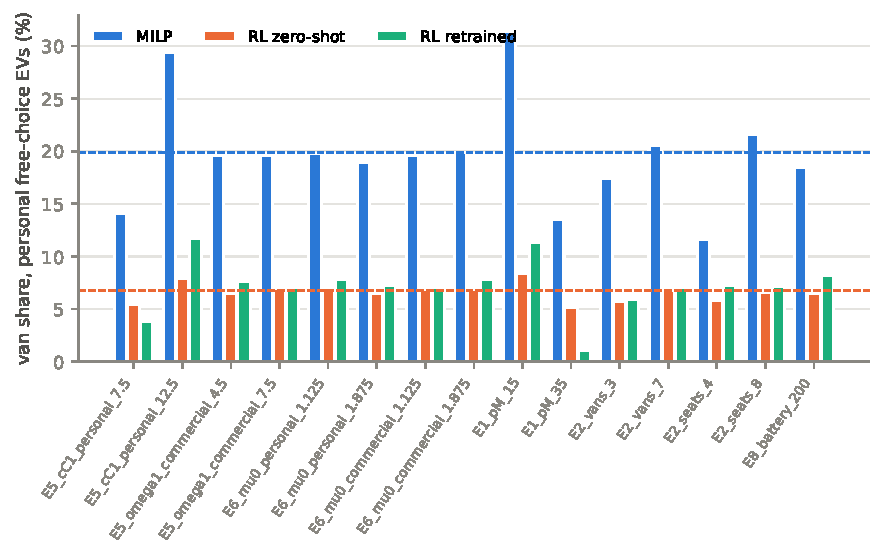
\includegraphics[width=0.95\textwidth]{figures/exp_vanshare.pdf}
\caption{Personal van share for every E1--E8 variant (MILP, RL zero-shot, RL retrained); dashed lines are the
baseline. Levers of price and of personal time move it; levers of money sensitivity and downtime do not.}
\label{fig:vanshare}
\end{figure}

\inshort{To estimate the \emph{cost}, the energy per car, the station power and how poor taxi drivers feel money
matter most. To decide \emph{who gets a van}, the van tariff and the personal value of station time are the tools;
the fleet size and battery decide only which instances can be served at all.}

%=====================================================================
\section{Validation: why the numbers can be trusted}
\label{sec:validation}

The report rests on three independent kinds of support, over and above each proposition's derivation.

\subsection{A direction the optimiser cannot violate}
Some directions are certain from the model alone: a dearer van tariff can never lower the \emph{optimal} cost
(every plan gets dearer); more vans, seats or battery can never raise it (every old plan is still allowed). On the
instances proven \emph{optimal in both} the baseline and the variant, the measured change must have the right sign.

\begin{table}[H]\centering
\caption{Direction check on instances proven optimal in both runs (MILP).}
\label{tab:direction}
\footnotesize
\begin{adjustbox}{max width=\linewidth}
\begin{tabular}{@{}lrrrr@{}}
\toprule
variant & $Z$ at the optimum & optimal in both & mean $\Delta Z$ (\%) & wrong direction \\
\midrule
E1\_pM\_15 & must not rise & 225 & $-$4.448 & 0 \\
E1\_pM\_35 & must not fall & 276 & $+$4.069 & 0 \\
E5\_cC1\_personal\_7.5 & must not rise & 275 & $-$2.190 & 0 \\
E5\_cC1\_personal\_12.5 & must not fall & 252 & $+$1.951 & 0 \\
E5\_omega1\_commercial\_4.5 & must not rise & 275 & $-$2.506 & 0 \\
E5\_omega1\_commercial\_7.5 & must not fall & 275 & $+$2.496 & 0 \\
E6\_mu0\_personal\_1.125 & must not rise & 273 & $-$1.298 & 0 \\
E6\_mu0\_personal\_1.875 & must not fall & 276 & $+$1.299 & 0 \\
E6\_mu0\_commercial\_1.125 & must not rise & 272 & $-$6.449 & 0 \\
E6\_mu0\_commercial\_1.875 & must not fall & 275 & $+$6.457 & 0 \\
E2\_vans\_3 & must not fall & 275 & $+$0.000 & 0 \\
E2\_vans\_7 & must not rise & 273 & $-$0.000 & 0 \\
E2\_seats\_4 & must not fall & 275 & $+$1.297 & 0 \\
E2\_seats\_8 & must not rise & 263 & $-$0.156 & 0 \\
E8\_battery\_200 & must not rise & 274 & $-$0.036 & 0 \\
\bottomrule
\end{tabular}
\end{adjustbox}

\end{table}
All \fnVariants{} E1--E8 variants pass with \textbf{\fdirectionBad{} violations} in about 4\,000 pairs of optimal
plans. This is the strongest internal evidence that the model, the data changes and the solver runs are
consistent; the propositions of Part~IV are its explanation.

\subsection{Two independent methods agree}
\label{sec:milpvsrl}
The exact MILP and the learned policy are built and solved completely differently, yet scored by the same checker.
Figure~\ref{fig:agreement} plots the cost change each experiment produces, MILP against RL.

\begin{figure}[H]
\centering
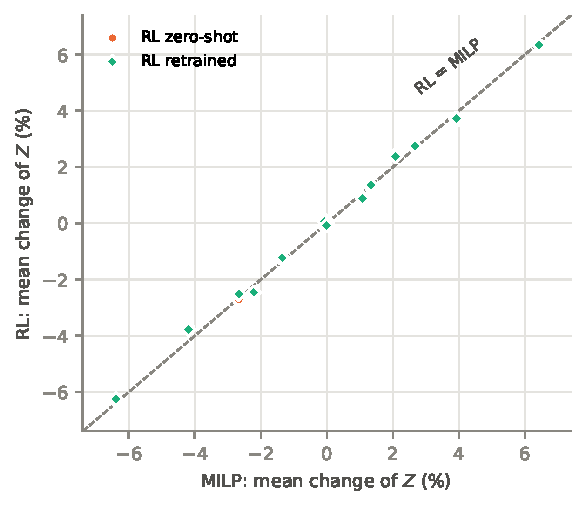
\includegraphics[width=0.56\textwidth]{figures/exp_agreement.pdf}
\caption{Mean $\Delta Z$ per variant: RL (zero-shot and retrained) against the MILP. Points on the diagonal mean
the two methods measure the same effect.}
\label{fig:agreement}
\end{figure}
The retrained RL agrees with the MILP to within \fagreeRtMean{} percentage points on average
(zero-shot \fagreeZsMean), and the sign agrees for all \fagreeSign{} of \fnVariants{} variants where the effect is
above noise. Because the two methods fail on \emph{different} instances (RL even places \frlOnlyFromNoPlan{} that
the MILP could not), their agreement on the \emph{effects} is not a shared bias --- it is confirmation.

\subsection{Theory, evidence and cause line up}
For every experiment the proposition's predicted direction, the measured number, and the practical mechanism point
the same way: E5 splits into an assignment lever and a level lever exactly as Proposition~\ref{prop:e5} says; E6's
size is read off the cost anatomy; E1, E2 and E8 obey the monotonicity/complementary-slackness arguments and the
direction check; E9 follows the charging-time law and E10 the affinity law, with the predicted asymmetry and
elasticity. When a derivation, two solvers and an operational story agree, the result is as well supported as this
kind of study allows.

\inshort{Every headline number is backed three ways: a direction the optimiser provably cannot break (0 violations
in 4\,000 optimal pairs), agreement of two independent methods (within \fagreeRtMean{} points), and a proposition
that predicts it.}

%=====================================================================
\section{Limitations}
\label{sec:limits}
\begin{itemize}
  \item \textbf{Placeholder sensitivities.} Apart from the segment share and the income distributions, the customer
  numbers are reasoned guesses; the experiments show \emph{how much} each matters, not its true value.
  \item \textbf{One change at a time.} Interactions (cheaper \emph{and} more vans, more demand \emph{and} more
  power) are not tested.
  \item \textbf{Time limit.} 223 of 560 baseline instances stop at 300\,s; effects smaller than the typical gap are
  read reliably only on the instances optimal in both (Table~\ref{tab:direction}).
  \item \textbf{Static demand.} All requests are known at time 0; real requests arrive during the day.
  \item \textbf{RL.} No optimality guarantee, one training run per model, and it under-uses vans, so the exact van
  policy is taken from the MILP. E9--E10 are RL-only (no MILP), justified by the close MILP--RL agreement on E1--E8.
  \item \textbf{Equity} is described (who queues, who pays, who feels what) but is not part of the objective.
\end{itemize}

%=====================================================================
\section{Conclusions}
\label{sec:concl}
\begin{enumerate}
  \item \textbf{Segment, not income, decides van use.} Vans are a service for rich \emph{private} owners; taxis
  take them only to escape a queue. This is rule \textbf{(T1)}--\textbf{(T3)} and it holds across every experiment.
  \item \textbf{The cost is driven by energy and by the poor.} Charging demand ($\pm22$\,\%) and station power
  ($\pm12$--20\,\%) are the largest levers because most of $Z$ scales with the energy charged; among the customer
  tastes, how a poor taxi driver feels money ($\pm6.4$\,\%) dominates, because taxis are the majority and the
  tariff is the biggest cost.
  \item \textbf{Price sets who gets vans; capacity sets who can be served.} The van tariff and the personal value
  of station time move the van share; the fleet size, the guns and the power decide feasibility --- below a point
  they strand cars rather than merely cost money.
  \item \textbf{The results are trustworthy.} Two independent methods agree to a fraction of a per cent, every
  provable direction holds with zero violations, and each number has a proof behind it.
  \item \textbf{Modelling guidance.} Van recharging can be dropped (E8). Effort to measure parameters should go
  first to the energy demand, the station power, and the commercial money sensitivity and downtime rate.
\end{enumerate}

\inshort{Formulation~4's one new fact --- personal versus commercial --- explains the whole plan: vans for rich
private owners, queues for taxis and the poor. Cost is governed by energy, power and the majority's money
sensitivity; feasibility by capacity. Every conclusion is backed by theory, by two agreeing methods, and by a
direction the optimiser cannot break.}

\vfill
{\footnotesize\emph{Reproducibility.} All figures, tables and numbers in this report are generated from the result
files by \code{report/make\_report\_f4.py} (which writes \code{figures/}, \code{tables/}, \code{numbers.tex});
the document is \code{report/analysis\_report\_f4.tex}. Every plan, from either method, is scored by the same
independent checker of constraints (2)--(23) and objective~\eqref{eq:obj}.}
